\documentclass[12pt]{article}

% URLs and hyperlinks ---------------------------------------
\usepackage{hyperref}
\hypersetup{
	colorlinks=true,
	linkcolor=blue,
	filecolor=magenta,      
	urlcolor=blue,
}
\usepackage{xurl}
%---------------------------------------------------

\usepackage{float}
\usepackage{adjustbox}
\usepackage{graphicx}
\usepackage{rotating}
\usepackage{mathtools}
\usepackage{enumitem}
\usepackage{gensymb}

\usepackage{xepersian}
\settextfont{Yas}

\title{گزارش کار آزمایش هفتم}
\author{	گروه: \\	اریسا احسانی \\	سید حسین حسینی \\	مهدی حق‌وردی \\ \\	شعبه شش
}
\date{}
\renewcommand{\arraystretch}{1.4}

\begin{document}
	\maketitle
	\tableofcontents
	\newpage
	
\section{}
\begin{figure}[H]
\begin{center}
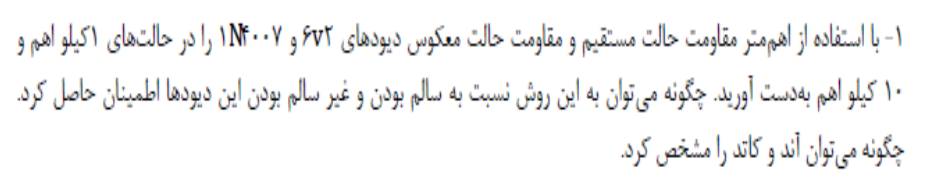
\includegraphics[width=\textwidth, height=3cm]{./images/7.1}
\end{center}
\end{figure}
	
در حالتی که دو طرف یک دیود جریان طبیعی خود را داشته باشد، به آن حالت مستقیم و در صورتی که ولتاژ در سراسر دیود در جهت متفاوت باشد، حالت معکوس اتفاق می‌وفتد.

ولتاژ موجود در یک دیود در حالت معکوس جیران قابل توجهی را تولید نمی‌کند (در حالت ایده‌آل اصلا نباید جریانی تولید شود) و از این ویژگی خاص برای تبدیل جریان متناوب به جریان مستقیم استفاده می‌شود.

در حالت مستقیم مانع بالقوه درون دیود ضعیف می‌شود تا جریان به نحو بهتری عبور کند و در حالت معکوس مانع بالقوه درون دیود قوی می‌شود که با حداکثر توان جلوی عبور جریان گرفته شود.

در دیود‌ها دو پایه‌ی مختلف وجود دارد که پایه‌ی بلند‌تر آند و آن پایه کاتد دیود است. سالم یا خراب بودن دیود‌ها را می‌توان با مولتی‌متر بررسی کرد.


\section{}
\begin{figure}[H]
	\begin{center}
		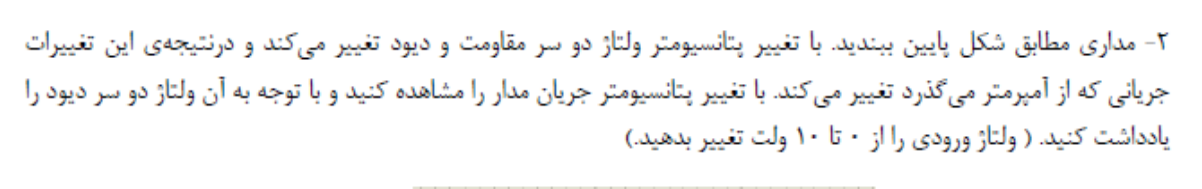
\includegraphics[width=\textwidth, height=3cm]{./images/7.2}
	\end{center}
\end{figure}

\begin{figure}[H]
	\begin{center}
		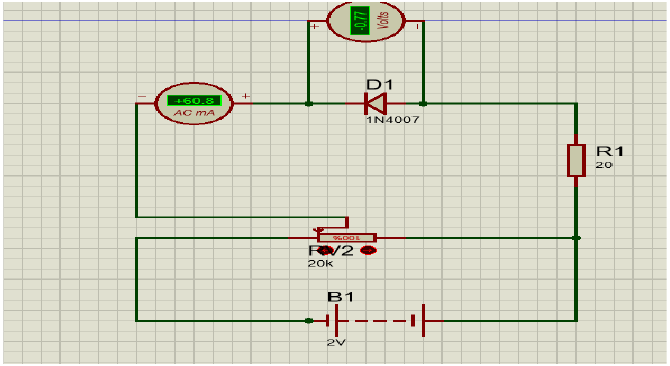
\includegraphics[width=\textwidth, height=8cm]{./images/7.3}
	\end{center}
\end{figure}

\begin{figure}[H]
	\begin{center}
		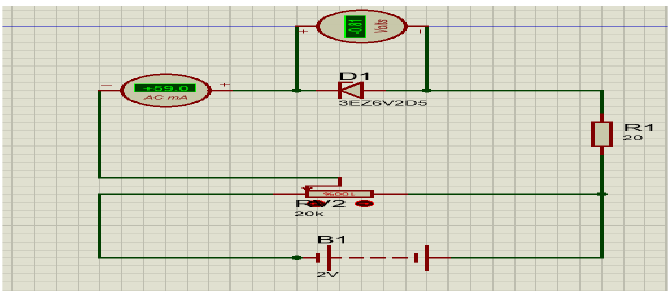
\includegraphics[width=\textwidth, height=8cm]{./images/7.4}
	\end{center}
\end{figure}

\begin{latin}
\begin{table}[H]
\begin{adjustbox}{width=\textwidth}
\begin{tabular}{|c|c|c|c|c|c|c|c|c|c|c|c|c|c|}
\hline
$I_D \, mA$ & 0 & 0.05 & 0.1 & 0.2 & 0.3 & 0.5 & 0.7 & 1 & 3 & 5 & 10 & 20 & 40 \\
\hline
\hline
$V_D (1N 4007) $ &
0.37 &
0.45 & 
0.48 & 
0.51 & 
0.53 & 
0.55 & 
0.57 & 
0.60 & 
0.63 & 
0.65 & 
0.68 & 
0.72 & 
0.75 \\
\hline
$V_D (z6v2) $ &
0.56 &
0.61 & 
0.63 & 
0.64 & 
0.65 & 
0.67 & 
0.68 & 
0.69 & 
0.72 & 
0.73 & 
0.75 & 
0.78 & 
0.80 \\
\hline
\end{tabular}
\end{adjustbox}
\end{table}
\end{latin}

\begin{figure}[H]
	\begin{center}
		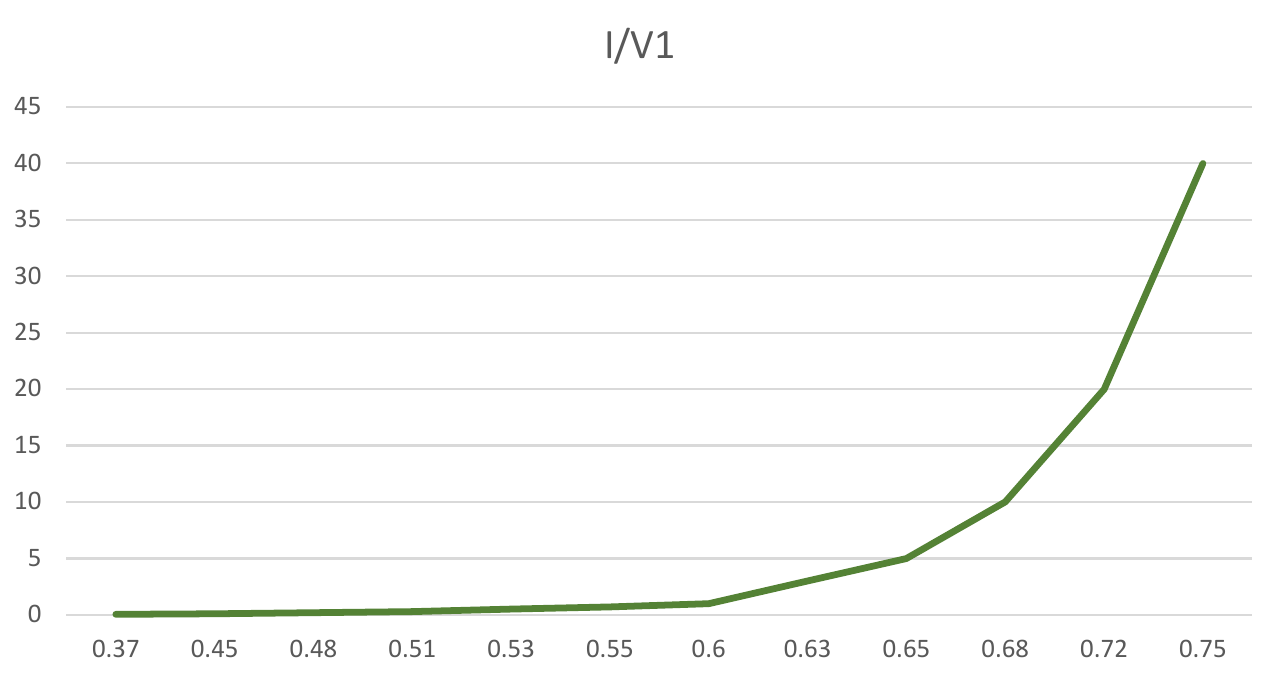
\includegraphics[width=\textwidth, height=8cm]{./images/7.5}
	\end{center}
\caption{نمودار جریان بر حسب ولتاژ دیود اول}
\end{figure}


\begin{figure}[H]
	\begin{center}
		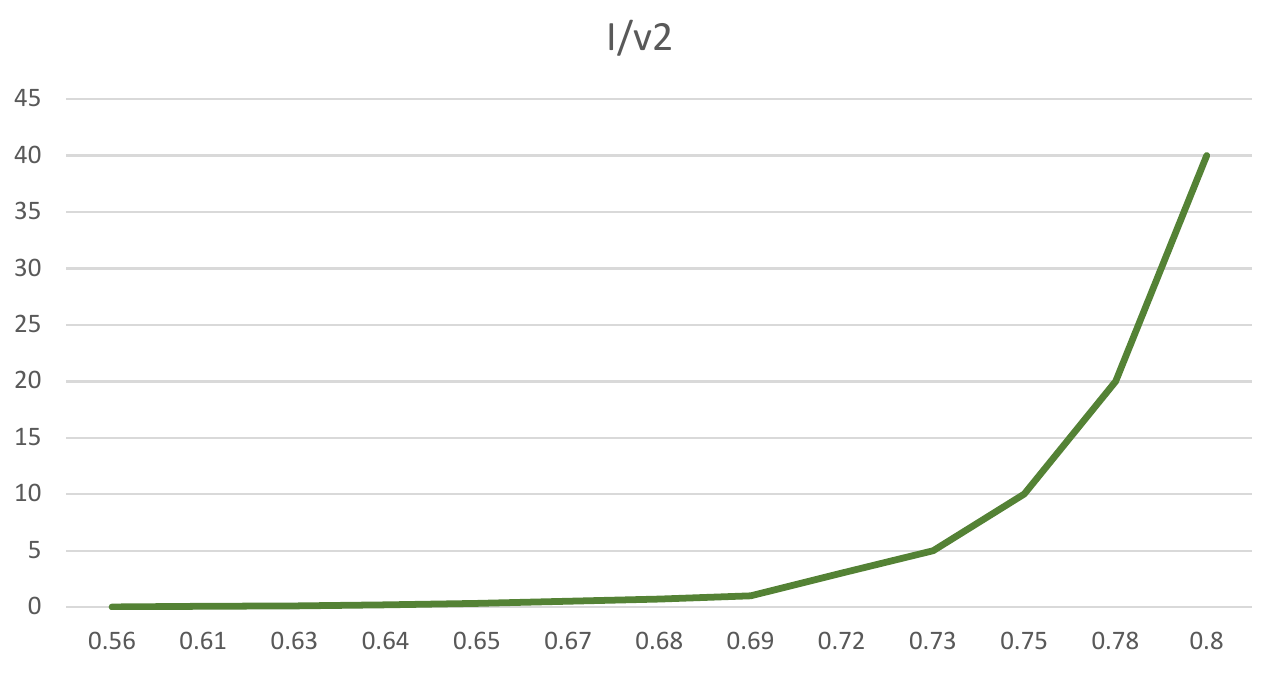
\includegraphics[width=\textwidth, height=8cm]{./images/7.6}
	\end{center}
\caption{نمودار جریان بر حسب ولتاژ دیود دوم}
\end{figure}


\section{}
\begin{figure}[H]
	\begin{center}
		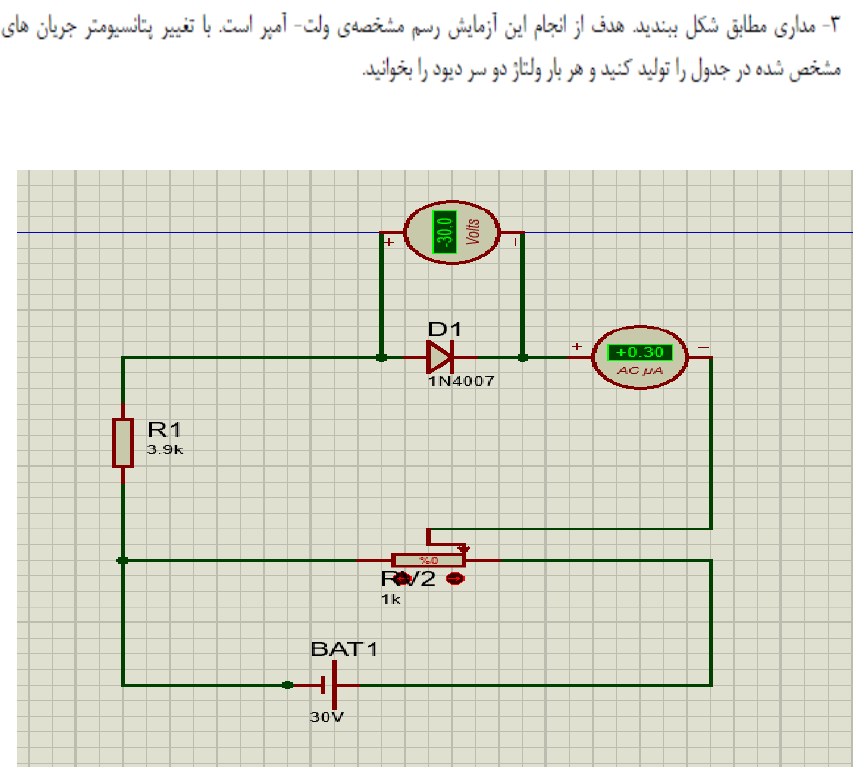
\includegraphics[width=\textwidth, height=12cm]{./images/7.7}
	\end{center}
\end{figure}

\begin{latin}
\begin{table}[H]
\begin{adjustbox}{width=\textwidth}
\begin{tabular}{|c|c|c|c|c|c|c|c|c|c|c|}
\hline
$V_D$ & 0 & 0.5 & 1 & 3 & 5 & 10 & 15 & 20 & 25 & 30 \\
\hline
\hline
$I_D \ \mu A$ & 0 & 0 & 0.01 & 0.03 & 0.05 & 0.1 & 0.15 & 0.2 & 0.25 & 0.3 \\
\hline
\end{tabular}
\end{adjustbox}
\end{table}
\end{latin}

\begin{latin}
\begin{table}[H]
\begin{adjustbox}{width=\textwidth}
\begin{tabular}{|c|c|c|c|c|c|c|c|c|c|}
\hline
$V_D$ & 0 & 0.3 & 0.5 & 1.5 & 3 & 3.5 & 4 & 4.5 & 5\\
\hline
\hline
$I_D \ \mu A$ & 0 & 0 & 0 & 0.01 & 0.03 & 0.03 & 0.04 & 0.04 & 0.05 \\
\hline
\end{tabular}
\end{adjustbox}
\end{table}
\end{latin}

\begin{figure}[H]
	\begin{center}
		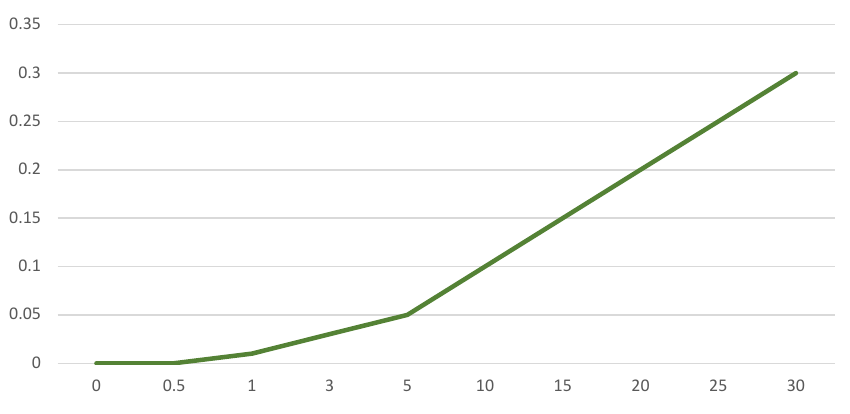
\includegraphics[width=\textwidth, height=6cm]{./images/7.8}
	\end{center}
\end{figure}

\begin{figure}[H]
	\begin{center}
		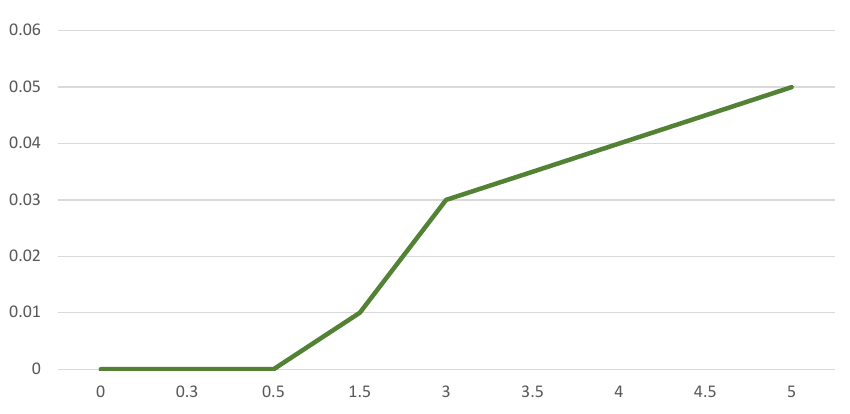
\includegraphics[width=\textwidth, height=6cm]{./images/7.9}
	\end{center}
\end{figure}

\section{}

\begin{figure}[H]
	\begin{center}
		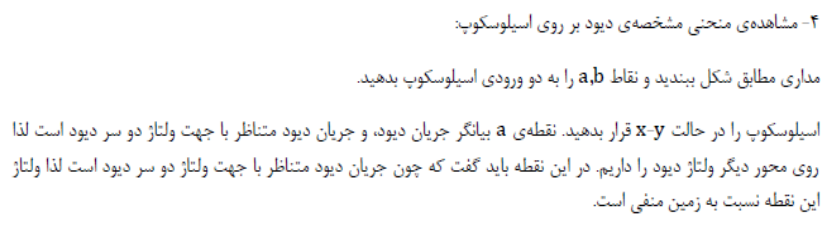
\includegraphics[width=\textwidth, height=6cm]{./images/7.10}
	\end{center}
\end{figure}

\begin{figure}[H]
	\begin{center}
		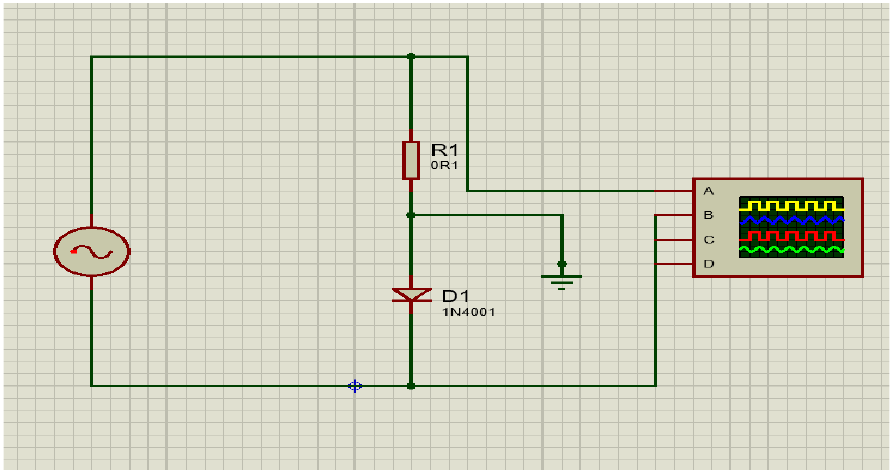
\includegraphics[width=\textwidth, height=8cm]{./images/7.11}
	\end{center}
\end{figure}

\begin{figure}[H]
	\begin{center}
		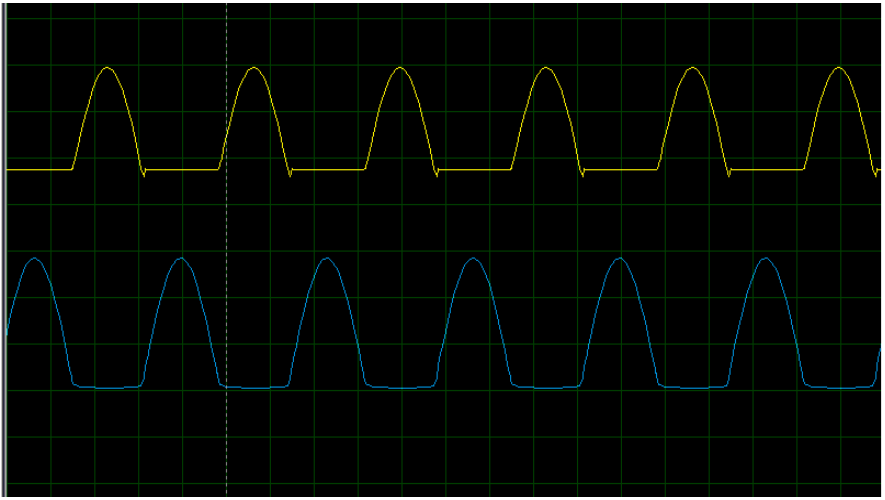
\includegraphics[width=\textwidth, height=7cm]{./images/7.12}
	\end{center}
\end{figure}

\end{document}